%%% Preamble
\documentclass[11pt]{article}

\usepackage[paper=A4,pagesize]{typearea}
\usepackage[utf8]{inputenc}
\usepackage[T1]{fontenc}
\usepackage[a4paper,pdftex]{geometry}	% Use A4 paper margins
\usepackage[french]{babel}
\usepackage{xcolor} % Required for specifying custom colors
\usepackage{fix-cm} % Allows increasing the font size of specific fonts beyond LaTeX default specifications
\usepackage{hyperref}
\usepackage{todonotes}
\usepackage{wrapfig}
\usepackage{pdfpages}
\usepackage{afterpage}
\usepackage{csvsimple}
\usepackage{float}
\restylefloat{table,figure}

%%  ========   IMPORTANT ========
%% Indiquer ici les parties que vous voulez compilez

%%% Begin document
\begin{document}
\includepdf[pages={1}]{title.pdf}

\listoftodos[Modifications du rapport]
\newpage

\tableofcontents

\listoffigures

\listoftables

\newpage

\section{Introduction}

\todo{Introduction ici}

\newpage

\section{Grammaire du langage lutin}

\todo{Grammaire du langage ici}

\newpage

\section{Automate LR}

\todo{Scan du diagramme de l'automate LR ici}

\newpage

\section{Table des transitions LR}

\todo{Table des transitions ici}

\newpage

\afterpage{
	\clearpage
	\KOMAoptions{paper=A3,pagesize,paper=landscape,DIV=20}
	\recalctypearea
	\section{Structures de données}
	\vspace{5cm}
	\begin{figure}[h]
		\centering
		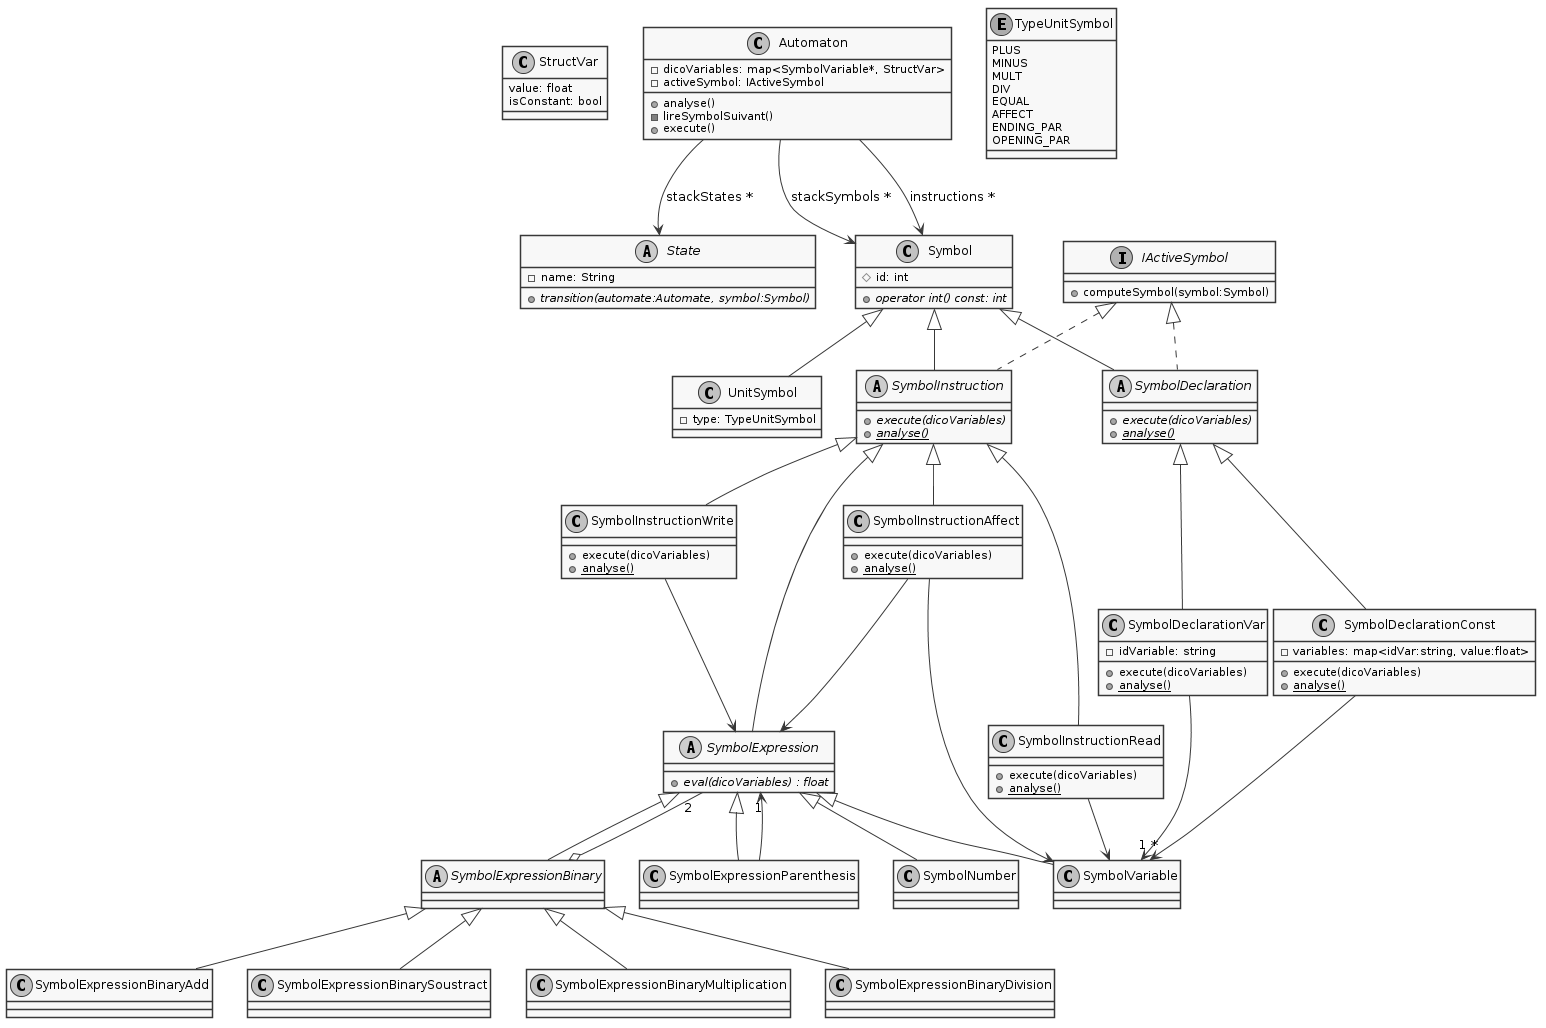
\includegraphics[width=1.0\textwidth,keepaspectratio]{../diagrams/class/lutin-compiler-class-diagram-uml.png}
		\caption{A large image which required A3}
	\end{figure}

	\clearpage
	\KOMAoptions{paper=A4,pagesize}
	\recalctypearea
}

%%% End document
\end{document}
